\chapter{\textsc{PathObjects} for Squeak Smalltalk}
\label{c:implementation}

\todo[inline]{Introduction}

\section{Data Acquisition}
\todo[inline]{Introduction}

\subsection{Identification of Objects}
\label{ImplementationTracingIdentification}

\subsection{Tracing Approach}
\label{ss:ImplementationTracingApproach}

\begin{figure}
	\centering
	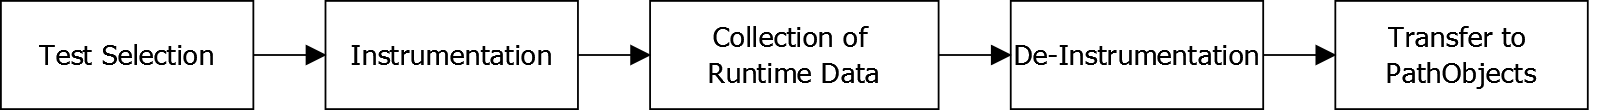
\includegraphics[width=0.9\textwidth]{../images/04-Tracing}
	\caption[TOC Caption]{Tracing foo}
	\label{fig:ImplementationTracing}
\end{figure}

Figure \ref{fig:ImplementationTracing} depicts the fundamental steps that are performed by the \textsc{PathTools} tracing framework to generate an execution trace.
First, the user selects a test case she wishes to analyze.
For instance, this can be done through the test coverage information 

In order to be suitable for the purposes of \textsc{PathObjects}, the tracing framework had to be extended in two places.
First, a custom \inlinecode{MethodWrapper} had to be implemented that collects the information required for the reconstruction of object interactions.
For each wrapped executed method, this specialized wrapper reports integer identifiers of the receiving object, of the method arguments, and of the return value to the tracer.
Thereby, argument objects are flattened.
That means that if collections of objects are used as arguments, the identifiers of the objects contained in a collection are reported in addition to the identifier of the collection object itself.
Note that an identifier for the sender of a message is not captured, since it would require the expensive operation of stack inspection.
However, this information can be easily reconstructed from the tree structure of the traces, since the sender of a message is identical to the parent element of a call node in the call tree.

The second extension that had to be made is the implementation of a custom \inlinecode{Tracer} that provides some functionality required by our method wrappers and for additional refinement runs.


\subsection{Reference Tracing}
\label{ss:ImplementationTracingReferences}

\section{Analyses}

\section{Visualization}
\subsection{Graph Layouting}
\subsection{Information Layers}